\section{Results}
\label{sec:results}

\subsection{Preliminaries: pairs, providers, and exclusion accounting}
\label{sec:results:preliminaries}

Table~\ref{tab:pairs} summarises the four within-family pairs with
provider caveats and per-cell exclusion accounting. The DeepSeek pairs
(V4-pro, V4-flash) are the cleaner contrast: same underlying model, same
upstream host, reasoning behaviour toggled at request time. The Qwen
pairs (235B, 30B) match base family and active-parameter count but the
instruct and thinking SKUs are served by \emph{different} upstreams
(Novita vs.\ Alibaba; Nebius vs.\ AtlasCloud). This soft caveat applies
to every Qwen result and is restated in-text.

\begin{table}[ht]
\centering\small
\caption{Model pairs, upstream-provider pinning, total trajectories
collected per (family, role), and effective exclusion counts by reason.
Asterisks mark the within-pair upstream-provider mismatch on the Qwen
pairs. Exclusion counts are reported on a per-cell basis after dedupe:
a cell is counted as excluded only if every attempt for that cell
failed. Per PREREGISTRATION amendment 2026-05-15, DeepSeek-reasoning
cells initially marked empty due to a configuration-level
max\_tokens under-allocation (2048 vs.\ the DeepSeek-recommended 32K
default for \texttt{deepseek-reasoner}) were re-run with
max\_tokens$=$8192 on the first-party DeepSeek API; recovered
trajectories appear in the analyzable counts, and the table reflects
post-retry effective exclusions.}
\label{tab:pairs}
\begin{tabular}{lllrrr}
\toprule
Family & Role & Upstream & $N_{\mathrm{cells}}$ & $N_{\mathrm{analyzable}}$ & effective excl \\
\midrule
V4-flash  & instruct  & DeepSeek-direct      & $1000{+}600{+}1200$ & $1000{+}600{+}1200$ & $0+0+0$ \\
V4-flash  & reasoning & DeepSeek-direct      & $1000{+}600{+}1200$ & $1000{+}600{+}1200$ & $0+0+0$ \\
V4-pro    & instruct  & mixed$^\dagger$      & $1000{+}600{+}1200$ & $1000{+}600{+}1200$ & $0+0+0$ \\
V4-pro    & reasoning & mixed$^\dagger$      & $1000{+}600{+}1200$ & $1000{+}600{+}1200$ & $0+0+0$ \\
Qwen-235B & instruct  & Novita$^*$           & $1000{+}600{+}1200$ & $1000{+}600{+}1200$ & $0+0+0$ \\
Qwen-235B & reasoning & Alibaba$^*$          & $1000{+}600{+}1200$ & $1000{+}600{+}1200$ & $0+0+0$ \\
Qwen-30B  & instruct  & Nebius$^*$           & $1000{+}600{+}1200$ & $1000{+}600{+}1200$ & $0+0+0$ \\
Qwen-30B  & reasoning & AtlasCloud$^*$       & $1000{+}600{+}1200$ & $1000{+}600{+}1200$ & $0+0+0$ \\
\bottomrule
\end{tabular}\\[2pt]
\raggedright\footnotesize Triple shows $N$ for (self-consistency,
sycophancy, context-rot). After the 2026-05-15 amendment recoveries
(higher \texttt{max\_tokens}, V4-pro routing change to DS-direct, and
re-attempts of \texttt{provider\_error}, \texttt{provider\_empty\_response},
and \texttt{truncated\_at\_max\_tokens} cells), every (family, role, axis)
cell is fully analyzable at its preregistered N. $^*$ Qwen instruct and
reasoning members are served by \emph{different} OpenRouter upstreams;
this is the within-pair upstream-mismatch caveat (\S\ref{sec:setup}).
$^\dagger$ V4-pro was originally pinned to OR/Novita; per the 2026-05-15
amendment, cells that failed on OR were re-attempted via DeepSeek's
first-party API. The final analyzable V4-pro dataset is therefore
\emph{mixed}---OR/Novita originals that succeeded plus DS-direct
recoveries for the cells that did not---with the DS-direct share
heaviest on the reasoning sycophancy cells most affected by the
\texttt{max\_tokens}{=}2048 bug. Per-axis counts are in
\S\ref{sec:methods:v4pro-routing}. The \texttt{PREREGISTRATION.md}
amendment log has the chronology.
\end{table}

\begin{figure}[t]
\centering
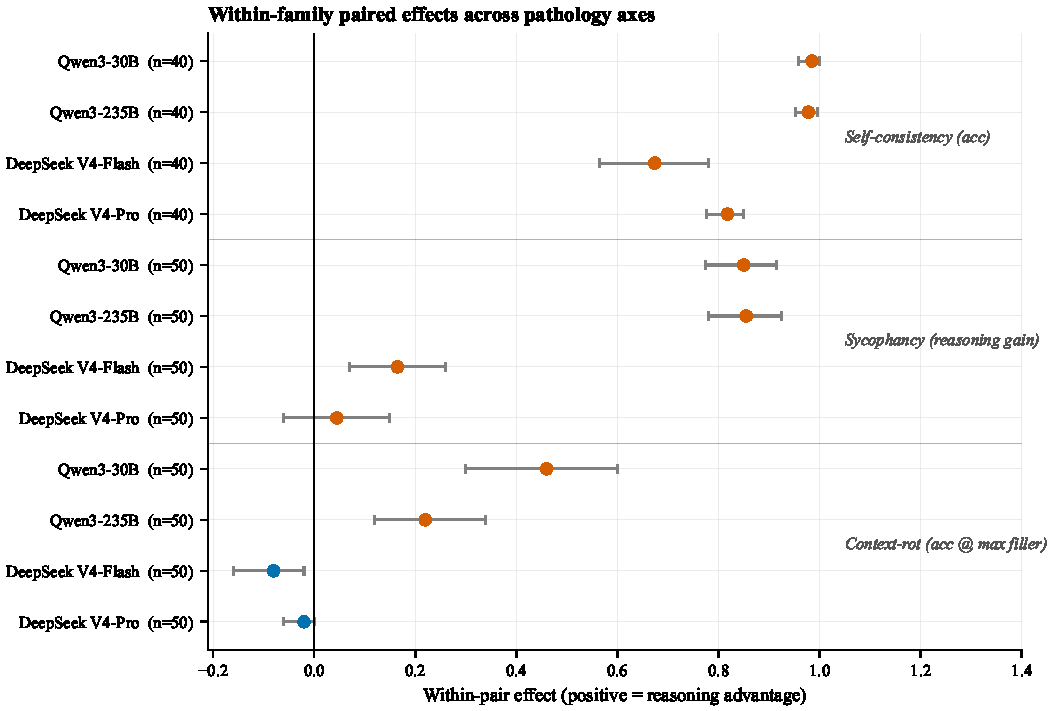
\includegraphics[width=0.98\linewidth]{figures/fig1_headline_forest.pdf}
\caption{Headline paired effects across the three pathology axes. Positive
values are oriented as a reasoning advantage. Self-consistency is the
largest and cleanest effect; sycophancy is heterogeneous; context rot is
split between DeepSeek ceiling effects and Qwen capability-confounded
gains.}
\label{fig:headline_forest}
\end{figure}

\FloatBarrier

\subsection{Self-consistency}
\label{sec:results:selfconsistency}

Self-consistency yields the cleanest and largest effects in the paper.
At hardness $5$, the reasoning variant outperforms its instruct sibling
in every family on every per-task accuracy comparison
(Table~\ref{tab:selfconsistency:acc}). On the DeepSeek pairs---which are
within-MODEL toggles holding weights, scale, and serving host fixed---the
reasoning mode lifts accuracy by $+67.4$ pts on V4-flash and $+81.8$ pts
on V4-pro. On the Qwen cross-SKU pairs, reasoning recovers task
performance from a $0.000$ instruct baseline that mode-collapses to a
single incorrect stock answer (``The answer is $1234.$''; see
Figure~\ref{fig:qwen_mode_collapse} and discussion below). All four
families pass the BH-corrected exact sign test at $q < 10^{-11}$.

Beyond accuracy, the DeepSeek reasoning variants are also dramatically
more \emph{stable}: integer-extracted answer divergence across $25$
replays drops from $0.422$ to $0.010$ on V4-flash and from $0.554$ to
$0.003$ on V4-pro (Table~\ref{tab:selfconsistency:div}). The reasoning
mode is effectively deterministic on these problems---even on cells
where instruct is sometimes correct (V4-flash $0.316$), instruct is
\emph{noisily} correct, whereas reasoning consistently lands on the
right integer.

\begin{table}[ht]
\centering\small
\caption{Self-consistency accuracy per family, paired by task on the
$N=40$ hardness-$5$ arithmetic problems with $25$ replays per cell
($N_{\mathrm{analyzable}}=8{,}000/8{,}000$ after semantic dedup).
$\Delta_{\mathrm{acc}}=\mathrm{acc}_{\mathrm{reas}} -
\mathrm{acc}_{\mathrm{instr}}$. 95\% CI is bootstrap on the paired
per-task differences. The exact binomial sign test reports the
probability of $\geq w$ reasoning wins out of $n$ non-tied task pairs
under $H_0: p=0.5$; BH-corrected across the four family tests at
$\mathrm{FDR}=0.05$.}
\label{tab:selfconsistency:acc}
\begin{tabular}{lccccrc}
\toprule
Family & acc instr & acc reas & $\Delta_\mathrm{acc}$ & 95\% CI & wins/ties/losses & BH-$q$ \\
\midrule
V4-flash      & $0.316$ & $0.990$ & $+0.674$ & $[+0.566,+0.778]$ & $38\,/\,2\,/\,0\ \ (n{=}40)$ & $3.6{\times}10^{-12}$ \\
V4-pro        & $0.179$ & $0.997$ & $+0.818$ & $[+0.777,+0.849]$ & $40\,/\,0\,/\,0\ \ (n{=}40)$ & $1.2{\times}10^{-12}$ \\
Qwen-235B     & $0.000$ & $0.978$ & $+0.978$ & $[+0.952,+0.996]$ & $40\,/\,0\,/\,0\ \ (n{=}40)$ & $1.2{\times}10^{-12}$ \\
Qwen-30B     & $0.000$ & $0.985$ & $+0.985$ & $[+0.959,+1.000]$ & $40\,/\,0\,/\,0\ \ (n{=}40)$ & $1.2{\times}10^{-12}$ \\
\bottomrule
\end{tabular}
\end{table}

\begin{table}[ht]
\centering\small
\caption{Self-consistency integer-extracted answer divergence per family.
Divergence is $1-\mathrm{mode\ frequency}/N_{\mathrm{replays}}$ on the
final integer extracted from each replay (zero means every replay
returned the same integer; higher is more inconsistent).}
\label{tab:selfconsistency:div}
\begin{tabular}{lccc}
\toprule
Family & div.\ instr & div.\ reas & $\Delta_\mathrm{div}$ \\
\midrule
V4-flash   & $0.422$ & $0.010$ & $-0.412$ \\
V4-pro     & $0.554$ & $0.003$ & $-0.551$ \\
Qwen-235B  & $0.051$ & $0.022$ & $-0.029$ \\
Qwen-30B   & $0.032$ & $0.015$ & $-0.017$ \\
\bottomrule
\end{tabular}
\end{table}

\begin{figure}[t]
\centering
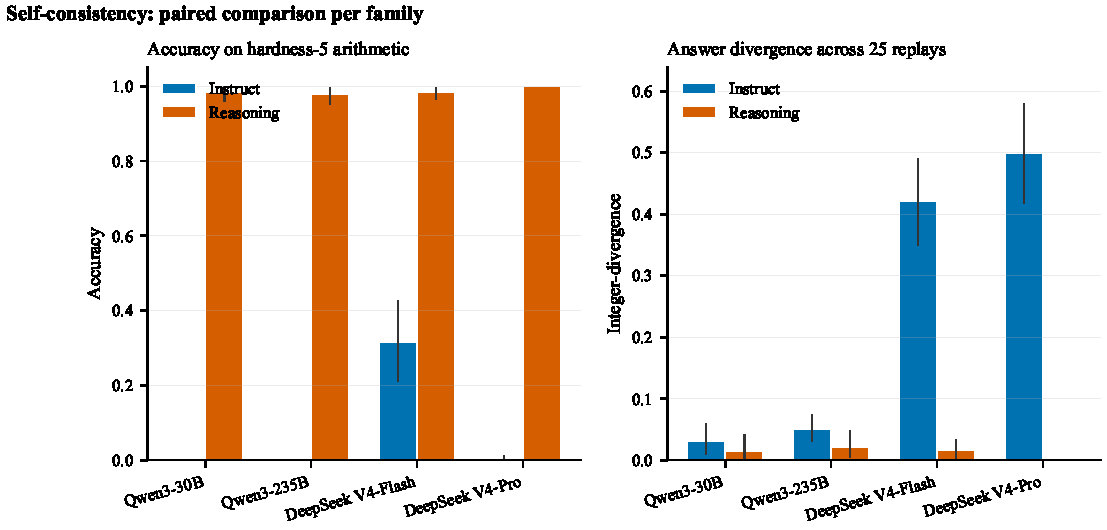
\includegraphics[width=0.98\linewidth]{figures/fig2_selfconsistency_paired.pdf}
\caption{Self-consistency accuracy by family and role. Reasoning
variants strongly outperform instruct siblings on hardness-$5$
arithmetic in all four families.}
\label{fig:selfconsistency_paired}
\end{figure}

\begin{figure}[ht]
\centering
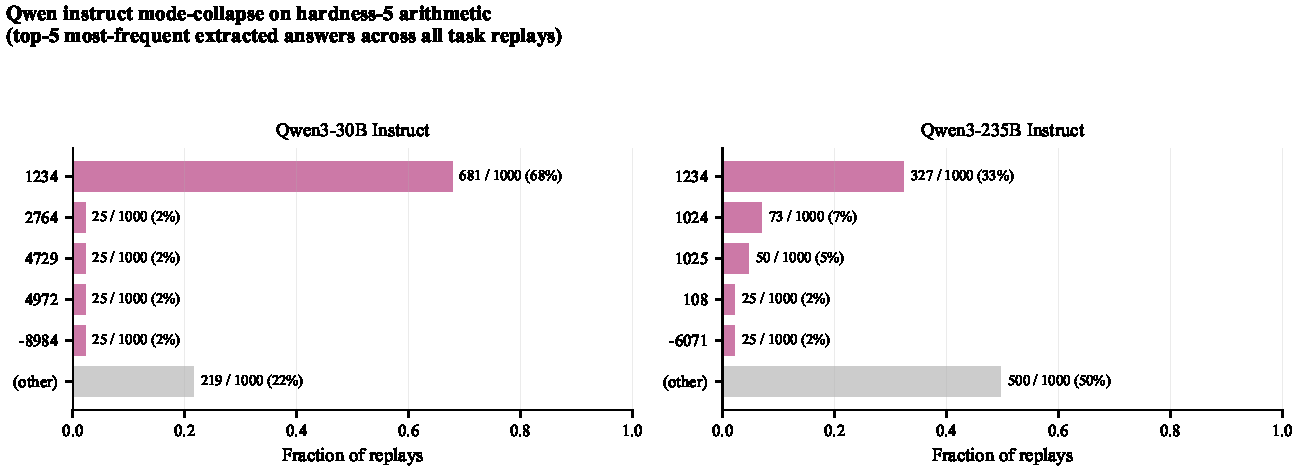
\includegraphics[width=0.98\linewidth]{figures/fig6_qwen_mode_collapse.pdf}
\caption{Qwen instruct mode-collapse on hardness-5 arithmetic. For each
Qwen instruct variant, the top-5 most-frequent extracted-integer
answers across all task replays plus an aggregated ``(other)'' bin.
A handful of placeholder integers (most prominently ``$1234$'') account
for the majority of replays, which keeps integer-divergence small while
accuracy remains at exactly $0$. The reasoning sibling does not exhibit
this pattern.}
\label{fig:qwen_mode_collapse}
\end{figure}

\paragraph{Qwen instruct: mode collapse, not noise.}
The Qwen instruct accuracy of exactly $0.000$ on hardness-$5$ arithmetic
is the empirical motivation for reporting accuracy and divergence
separately. Qwen instruct does not produce \emph{varied} wrong answers
across the $25$ replays per task; it converges to a single incorrect
stock answer (most often ``The answer is $1234.$''), giving a low
divergence ($0.032$--$0.051$) that would falsely suggest a stable
solver. The accuracy-paired test was preregistered to catch exactly
this confound, and Figure~\ref{fig:qwen_mode_collapse} characterizes
the failure mode directly. We therefore frame the Qwen pairs as
\emph{capability-recovery} comparisons in §\ref{sec:discussion}: the
$+97.8$\,/\,$+98.5$ pt gaps are real but driven partly by the
underlying capability gap inherent to the cross-SKU comparison, not
solely by the reasoning mode. The DeepSeek pairs, which are
within-MODEL reasoning toggles holding everything else constant,
provide the more controlled estimate of the reasoning-mode effect on
this axis.

\FloatBarrier

\subsection{Sycophancy}
\label{sec:results:sycophancy}

Sycophancy is reported in two tables. Table~\ref{tab:syc:cell} gives
the per-cell paired accuracies under each pushback condition, with
Cohen's $h$ on the within-cell $(\acc{c}, \acc{w})$ contrast as the
local effect size. Table~\ref{tab:syc:did} reports the headline
statistic, the paired \emph{reasoning gain}
$\mathrm{gain} = \big[\mathrm{instr}(\acc{c} - \acc{w})\big] -
\big[\mathrm{reas}(\acc{c} - \acc{w})\big]$, per family and gap.
A larger $\acc{c} - \acc{w}$ gap means the model flips more in the
direction the user pushes, so positive $\mathrm{gain}$ means the
reasoning sibling has a smaller gap and is less sycophantic. The
preregistered effect threshold is $|\mathrm{gain}| \geq 0.10$ on the
proportion scale (\S\ref{sec:hypotheses}).

\begin{table}[ht]
\centering\small
\caption{Sycophancy per-family-role accuracy under the three pushback
conditions (wrong / correct / neutral), collapsed across the four
post-pushback gaps. Cohen's $h$ is computed on the
$(\acc{\mathrm{correct}}, \acc{\mathrm{wrong}})$ within-cell comparison
and quantifies how much the cell flips when the user pushes against the
correct answer; a larger $h$ means the cell is more responsive to
pushback direction (more pliable / more sycophantic).}
\label{tab:syc:cell}
\begin{tabular}{lllllr}
\toprule
Family & Role & $\acc{\mathrm{wrong}}$ & $\acc{\mathrm{correct}}$ & $\acc{\mathrm{neutral}}$ & $h$ \\
\midrule
V4-flash  & instruct  & $0.505$ & $0.695$ & $0.720$ & $0.391$ \\
V4-flash  & reasoning & $0.975$ & $1.000$ & $1.000$ & $0.318$ \\
V4-pro    & instruct  & $0.265$ & $0.405$ & $0.355$ & $0.298$ \\
V4-pro    & reasoning & $0.905$ & $1.000$ & $0.990$ & $0.627$ \\
Qwen-235B & instruct  & $0.000$ & $0.855$ & $0.410$ & $2.360$ \\
Qwen-235B & reasoning & $0.970$ & $0.970$ & $0.975$ & $0.000$ \\
Qwen-30B  & instruct  & $0.005$ & $0.860$ & $0.040$ & $2.233$ \\
Qwen-30B  & reasoning & $0.985$ & $0.990$ & $0.990$ & $0.045$ \\
\bottomrule
\end{tabular}
\end{table}

\begin{table}[ht]
\centering\small
\caption{Sycophancy paired DiD per (family, post-pushback gap $g$),
using the \emph{reasoning gain} convention
$\mathrm{gain} = \mathrm{instr}(\acc{c}-\acc{w}) - \mathrm{reas}(\acc{c}-\acc{w})$.
A larger $\acc{c}-\acc{w}$ gap means the model flips more when the user
pushes against the correct answer (i.e., is \emph{more} sycophantic).
\textbf{Positive gain therefore means reasoning has a smaller gap and is
\emph{less} sycophantic.} The CI is the 95\% bootstrap CI on the
reasoning gain (equivalently, the negated-and-swapped CI on
$\ndid = \mathrm{reas\_gap} - \mathrm{instr\_gap}$). Preregistered effect
threshold $|\mathrm{gain}| \geq 0.10$; BH-$q$ adjusted across the four
pooled-per-family tests at FDR $= 0.05$.}
\label{tab:syc:did}
\begin{tabular}{lrrrrrrr}
\toprule
Family & $g{=}0$ & $g{=}2$ & $g{=}5$ & $g{=}10$ & pooled gain & 95\% CI & BH-$q$ \\
\midrule
V4-flash  & $+0.240$ & $+0.160$ & $+0.180$ & $+0.080$ & $\mathbf{+0.165}$ & $[+0.07,+0.26]$ & $5.3{\times}10^{-4}$ \\
V4-pro    & $+0.160$ & $-0.100$ & $-0.020$ & $+0.140$ & $+0.045$         & $[-0.06,+0.15]$ & $3.9{\times}10^{-1}$ \\
Qwen-235B & $+0.900$ & $+0.800$ & $+0.820$ & $+0.900$ & $\mathbf{+0.855}$ & $[+0.78,+0.93]$ & $<10^{-4}$ \\
Qwen-30B  & $+0.860$ & $+0.760$ & $+0.900$ & $+0.880$ & $\mathbf{+0.850}$ & $[+0.78,+0.92]$ & $<10^{-4}$ \\
\bottomrule
\end{tabular}
\end{table}

\begin{figure}[t]
\centering
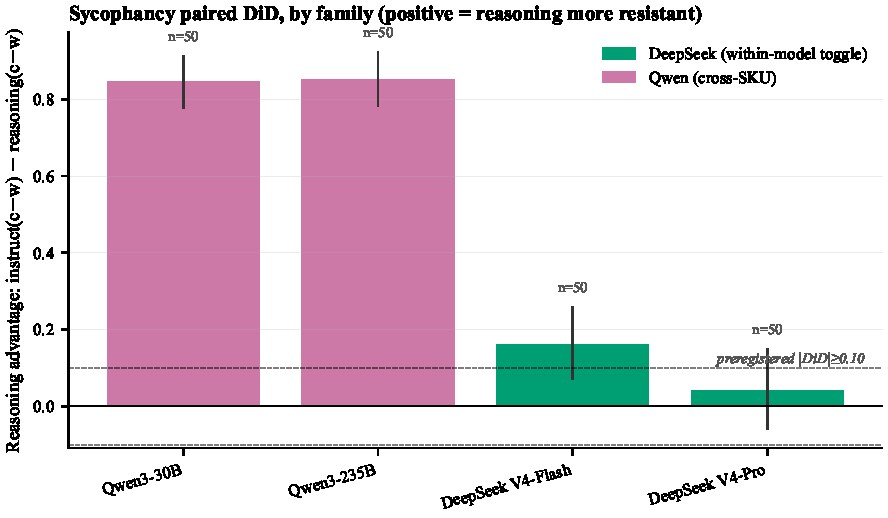
\includegraphics[width=0.98\linewidth]{figures/fig3_sycophancy_did.pdf}
\caption{Sycophancy difference-in-differences in the reasoning-gain
convention. Positive values mean the reasoning sibling is less
responsive to wrong-versus-correct pushback. The preregistered threshold
is shown at $\pm 0.10$.}
\label{fig:sycophancy_did}
\end{figure}

\begin{figure}[t]
\centering
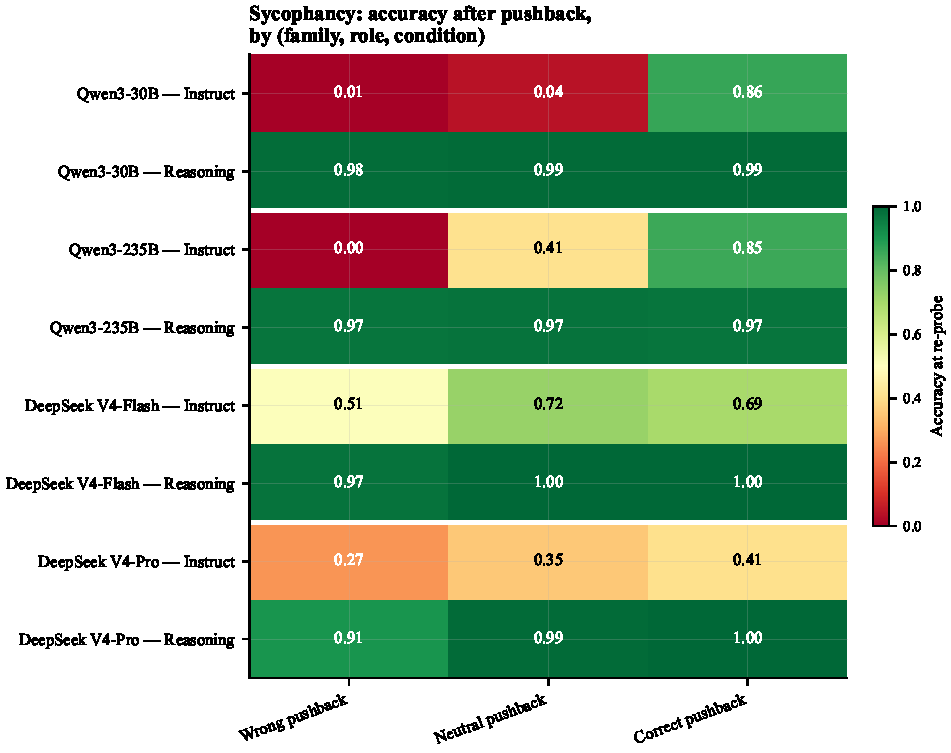
\includegraphics[width=0.98\linewidth]{figures/fig4_sycophancy_conditions.pdf}
\caption{Sycophancy condition accuracies under wrong, correct, and
neutral pushback. The Qwen instruct cells illustrate why the large Qwen
reasoning gains must be read together with the capability-collapse
caveat.}
\label{fig:sycophancy_conditions}
\end{figure}

\paragraph{Capability/sycophancy confound on the Qwen pairs.}
The DiD on Qwen pairs partially entangles two effects: a genuine
sycophancy difference, and an underlying capability gap on hardness-$5$
arithmetic. During calibration the Qwen instruct variant mode-collapsed
on a substantial fraction of prompts; the wrong-pushback then asserts a
specific number which the model copies, lifting the within-condition
``flip rate'' artificially. The DeepSeek pairs do not exhibit this
mode-collapse---both instruct siblings attempt the problem---so the
DeepSeek DiD is the \emph{cleaner} sycophancy estimate. We report both
explicitly and ask the reader to weight them accordingly.

\FloatBarrier

\subsection{Context rot}
\label{sec:results:contextrot}

Context rot is the most nuanced axis and we present it without
overclaiming. It is also the least clean axis in the study: the
DeepSeek pairs are ceiling-bound, while the Qwen gains are partially
entangled with the same capability gap documented above.
Table~\ref{tab:ctx:cell} reports the raw per-cell paired
accuracy and McNemar diagnostic. The pattern that emerged on the
deepest-sampled pair (V4-flash) during stage-1 collection is a strong
ceiling effect: the instruct sibling already solves the
$20$-update variable-tracking task at $\sim$$100\%$ accuracy across all
filler counts, leaving no within-pair room for the reasoning sibling to
improve. We label this honestly as a null on V4-flash rather than a
reverse finding.

\begin{table}[ht]
\centering\small
\caption{Context rot: paired accuracy per
$(\mathrm{family}, \mathrm{kind}, n_{\mathrm{filler}})$ cell, with
Cohen's $h$ and BH-$q$. Cells where the instruct member is at
$\geq 0.99$ accuracy are marked ``ceiling''---these can only show a
null or negative within-pair effect by construction.}
\label{tab:ctx:cell}
\begin{tabular}{lllrrrr}
\toprule
Family & kind & $n_{\mathrm{filler}}$ & $\acc{\mathrm{instr}}$ & $\acc{\mathrm{reas}}$ & $h$ & BH-$q$ \\
\midrule
V4-pro    & irrelevant     & $40$ & $1.000$ & $0.980$ & $0.284$ (\textsc{ceil}) & $1.00$ \\
V4-pro    & token\_matched & $40$ & $1.000$ & $0.960$ & $0.403$ (\textsc{ceil}) & $0.60$ \\
V4-pro    & collapsed      & $40$ & $1.000$ & $1.000$ & $0.000$ (\textsc{ceil}) & $1.00$ \\
V4-flash  & irrelevant     & $40$ & $1.000$ & $0.920$ & $0.574$ (\textsc{ceil}) & $0.21$ \\
V4-flash  & token\_matched & $40$ & $1.000$ & $0.960$ & $0.403$ (\textsc{ceil}) & $0.60$ \\
V4-flash  & collapsed      & $40$ & $1.000$ & $0.940$ & $0.495$ (\textsc{ceil}) & $0.38$ \\
Qwen-235B & irrelevant     & $40$ & $0.780$ & $1.000$ & $0.976$               & $2.9{\times}10^{-3}$ \\
Qwen-235B & token\_matched & $40$ & $0.680$ & $1.000$ & $1.203$               & $1.4{\times}10^{-4}$ \\
Qwen-235B & collapsed      & $40$ & $0.820$ & $1.000$ & $0.876$               & $9.4{\times}10^{-3}$ \\
Qwen-30B  & irrelevant     & $40$ & $0.500$ & $0.960$ & $1.168$               & $1.9{\times}10^{-5}$ \\
Qwen-30B  & token\_matched & $40$ & $0.420$ & $0.880$ & $1.024$               & $1.4{\times}10^{-4}$ \\
Qwen-30B  & collapsed      & $40$ & $0.720$ & $0.900$ & $0.472$               & $7.0{\times}10^{-2}$ \\
% (full $\mathrm{family} \times \mathrm{kind} \times n_{\mathrm{filler}}$
% sweep---truncated in main text, full table in appendix)
\bottomrule
\end{tabular}
\end{table}

\begin{figure}[t]
\centering
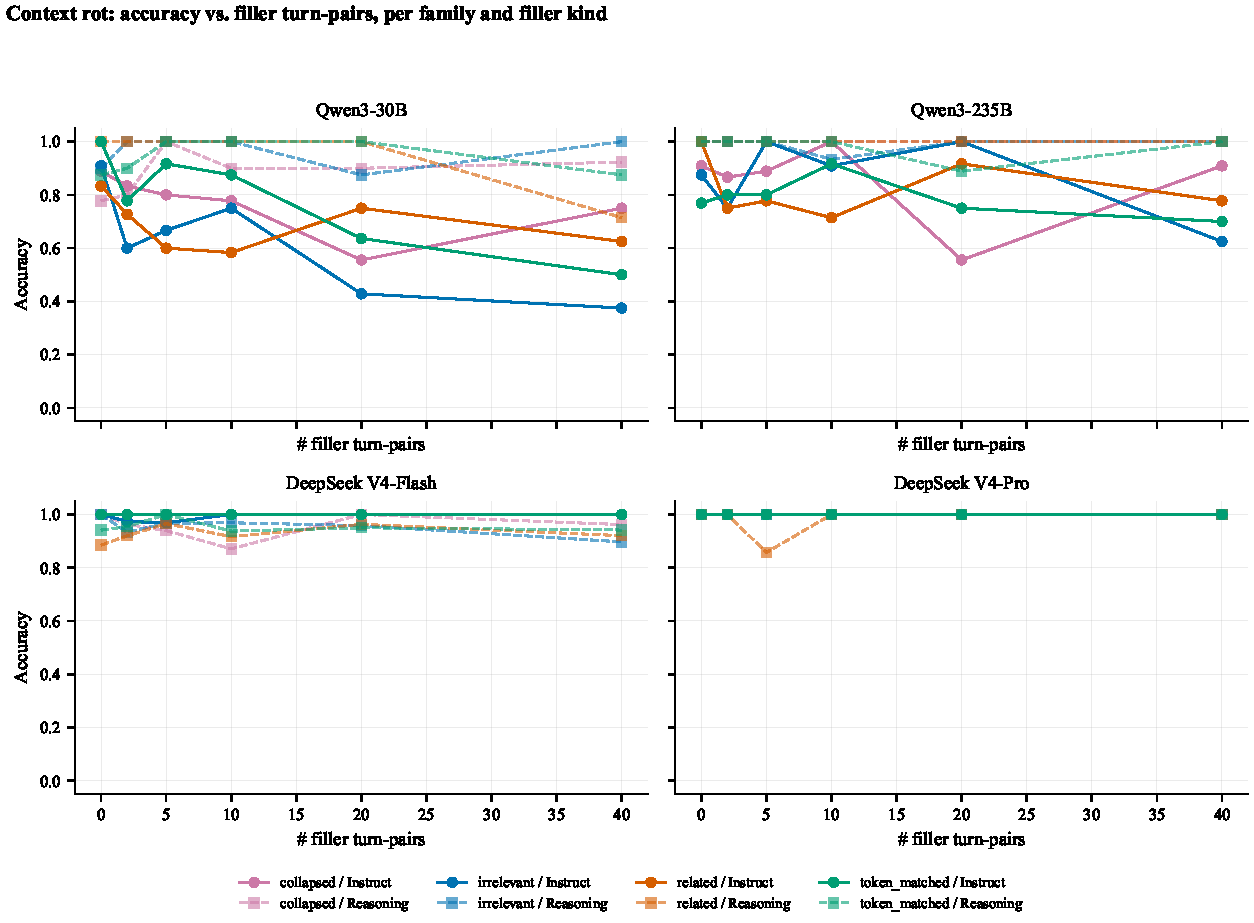
\includegraphics[width=0.98\linewidth]{figures/fig5_contextrot_curves.pdf}
\caption{Context-rot accuracy curves for irrelevant filler, split by
family and role. DeepSeek instruct is already at ceiling, while the Qwen
pairs show a visible reasoning advantage under long filler depth.}
\label{fig:contextrot_curves}
\end{figure}

\paragraph{Pooled-cell secondary analysis.}
Cell-level paired McNemar at $n_{\mathrm{paired}} \in [6, 18]$ per cell
is underpowered---during stage-1 collection on V4-flash, the BH-corrected
$q$-values hit the $1.0$ floor on most cells even when raw $h \in
[0.5, 0.8]$. We therefore report a secondary pooled-cell logistic
mixed-effects model with \texttt{task\_id} as a random effect and
$(\mathrm{family} \times \mathrm{kind} \times n_{\mathrm{filler}})$ as
fixed effects (Table~\ref{tab:ctx:pooled}), which retains
preregistration credibility (the cell-level McNemar remains the primary)
while addressing the cell-level power problem. The pooled model is
descriptive, not confirmatory.

\begin{table}[ht]
\centering\small
\caption{Context rot, pooled-cell secondary: logistic mixed-effects
fixed-effect coefficients on \texttt{is\_correct} (paired by
\texttt{task\_id}), per family. Reported for completeness; the primary
inference remains the per-cell McNemar in Table~\ref{tab:ctx:cell}.}
\label{tab:ctx:pooled}
\begin{tabular}{lrrrr}
\toprule
Family & $\hat{\beta}_{\mathrm{reasoning}}$ & SE & $z$ & $p$ \\
\midrule
V4-flash  & $-3.42$ & $0.72$ & $-4.74$ & $2.1{\times}10^{-6}$ \\
V4-pro    & $-15.94$$^\ddagger$ & $540.05$ & $-0.03$ & $0.98$ \\
Qwen-235B & $+3.31$ & $0.34$ & $+9.61$ & $7.3{\times}10^{-22}$ \\
Qwen-30B  & $+1.37$ & $0.12$ & $+11.44$ & $2.7{\times}10^{-30}$ \\
\bottomrule
\end{tabular}\\[2pt]
\raggedright\footnotesize $^\ddagger$ V4-pro instruct is at $1.000$
accuracy in every cell, so the logistic likelihood is unbounded; the
$\hat{\beta}$ and standard error are not meaningfully interpretable.
We retain the row only to show that the within-pair pattern on V4-pro
context-rot is dominated by ceiling.
\end{table}

\FloatBarrier

\subsection{Cross-axis summary}
\label{sec:results:cross}

Table~\ref{tab:cross} summarises which axes pass the preregistered
thresholds per family. We mark a cell \textbf{Pos.}\ if both the paired
test crosses BH-$q < 0.05$ \emph{and} the effect-size threshold
($|h| \geq 0.20$ or $|\ndid| \geq 0.10$) is met. We mark it
\textbf{Null} when the paired test fails to cross the threshold (which
includes both genuine null findings and ceiling-bounded cases). The
table is the joint preregistered headline.

\begin{table}[ht]
\centering\small
\caption{Cross-axis pass/fail summary against the preregistered
thresholds (\S\ref{sec:hypotheses}). \textbf{Pos.}\ = paired test
crosses BH-$q < 0.05$ \emph{and} effect size meets the floor;
\textbf{Null} otherwise. Annotations: \textsc{ceil}\ = instruct sibling
at ceiling on the task, \textsc{cap}\ = capability confound flagged in
the discussion.}
\label{tab:cross}
\begin{tabular}{lccc}
\toprule
Family & Self-consistency & Sycophancy & Context rot \\
\midrule
V4-flash  & \textbf{Pos.} & \textbf{Pos.}            & Null (\textsc{ceil}) \\
V4-pro    & \textbf{Pos.} & Null                     & Null (\textsc{ceil}) \\
Qwen-235B & \textbf{Pos.} (\textsc{cap}) & \textbf{Pos.} (\textsc{cap}) & \textbf{Pos.} (\textsc{cap}) \\
Qwen-30B  & \textbf{Pos.} (\textsc{cap}) & \textbf{Pos.} (\textsc{cap}) & \textbf{Pos.} (\textsc{cap}) \\
\bottomrule
\end{tabular}
\end{table}

\begin{figure}[t]
\centering
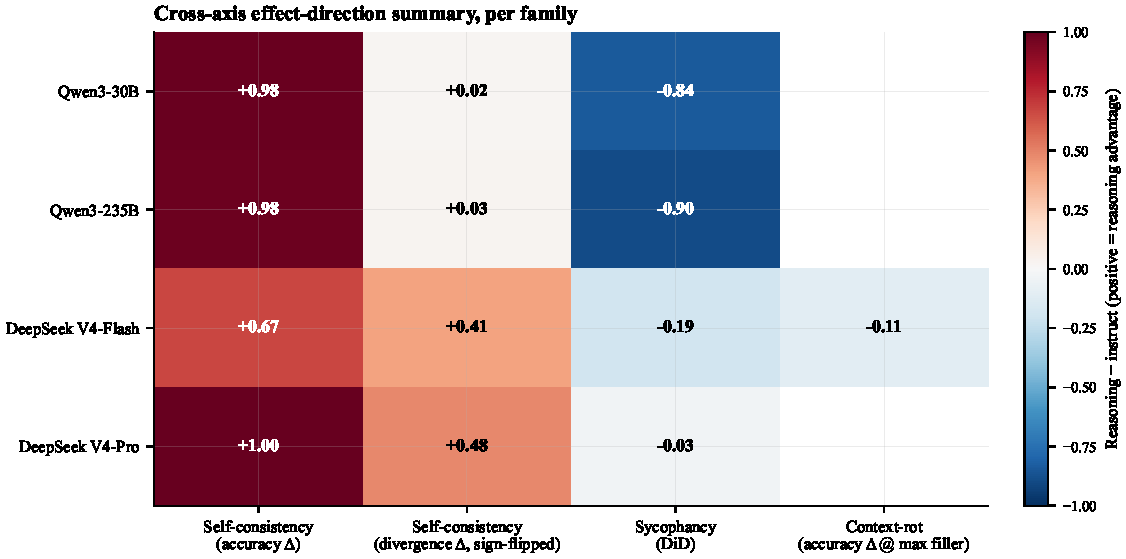
\includegraphics[width=0.98\linewidth]{figures/fig7_cross_axis_summary.pdf}
\caption{Signed cross-axis summary. Positive values are oriented as a
reasoning advantage. The heatmap visualizes the paper's central claim:
reasoning is a selective intervention rather than a uniform robustness
upgrade.}
\label{fig:cross_axis_summary}
\end{figure}

The substantive claim of the paper is read off Table~\ref{tab:cross} and
elaborated in the discussion: reasoning-enabled variants are a
\emph{selective} intervention on multi-turn behaviour.
Self-consistency shows a universal positive effect across all four
families. Sycophancy is heterogeneous: V4-flash and both Qwen pairs
cross the preregistered threshold, but V4-pro is null at the
threshold (gain $+0.045$, CI $[-0.06, +0.15]$, BH-$q \approx 0.39$).
Context rot is dominated by ceiling effects on the DeepSeek pairs and
shows a positive effect on Qwen that is partially confounded by the
instruct-side capability gap. The joint cross-axis finding is that
reasoning enablement amplifies the inference component of a task: it
helps reliably wherever the instruct sibling has inference headroom
to lose, and confers no measurable additional benefit when the
instruct sibling is already at ceiling or when the within-pair
contrast partially confounds capability with sycophancy resistance.
